\newpage

%%%%%%%%%%%%%%%%%%%%%%%%%%%%%%%%%%%%%%%%%%%%%%%%%%%%%%%%%%%%%%%%%%%%%%%%%%%%%%%%%%%%%%%
%%%%%%%%%%%%%%%%%%%%%%%%%%%%%%%%%%%%%%%%%%%%%%%%%%%%%%%%%%%%%%%%%%%%%%%%%%%%%%%%%%%%%%%
%%%%%%%%%%%%%%%%%%%%%%%%%%%%%%%%%%%%%%%%%%%%%%%%%%%%%%%%%%%%%%%%%%%%%%%%%%%%%%%%%%%%%%%
\section{Regressão logística e SE com classificador $f_{\VECTOR{c}}(x):~\mathbb{R} \rightarrow \mathbb{R}$}
\label{sec:theo:reglogr1r1:1}

\index{Regressão!Logística $f_{\VECTOR{c}}(x):~\mathbb{R} \rightarrow \mathbb{R}$}



\begin{theorem}[Classificação de dados em $\mathbb{R}$:]\label{theo:reglogr1r1:1}
~\\
\noindent
\begin{minipage}{0.45\textwidth}
\centering
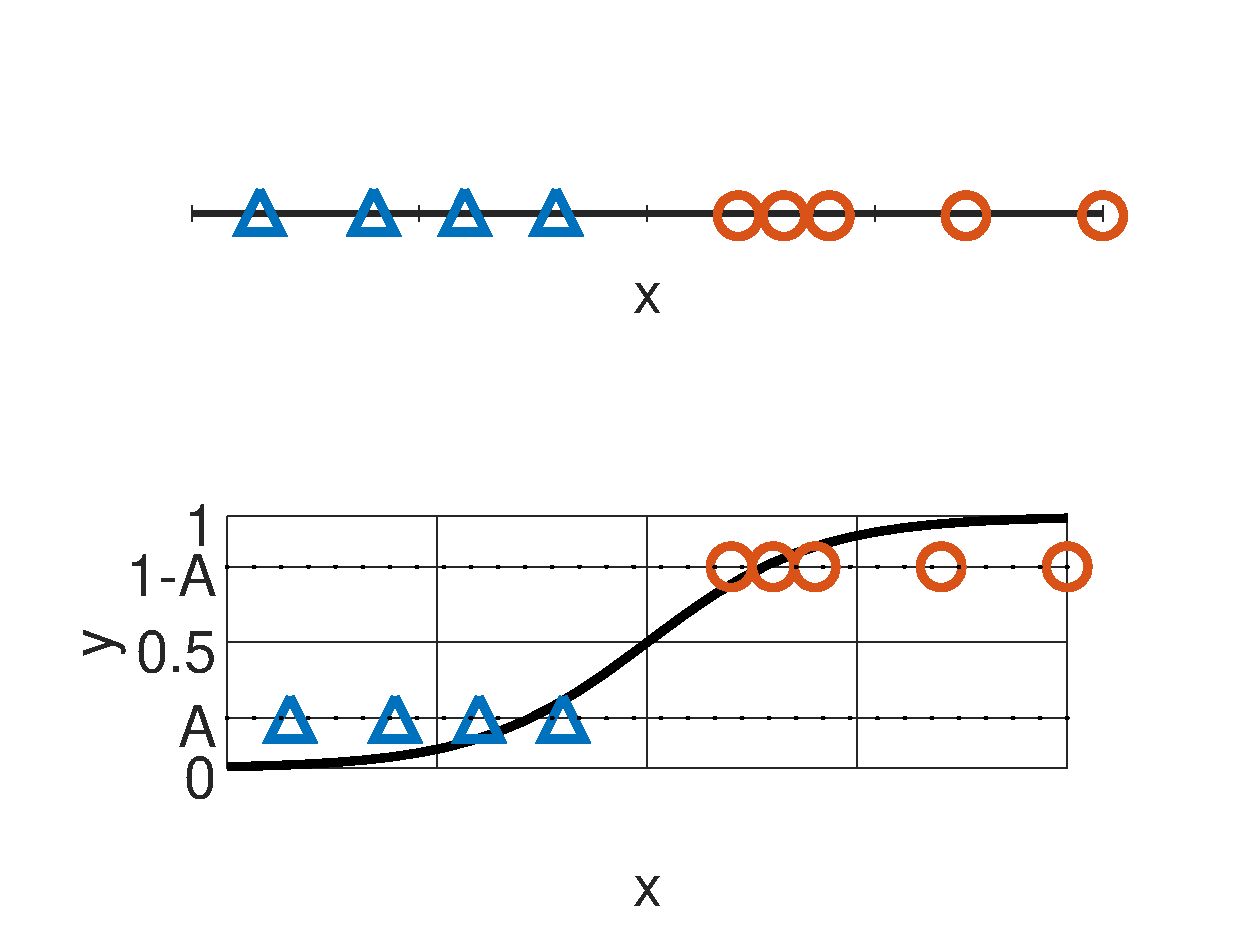
\includegraphics[width=0.95\linewidth]{chapters/classificacao/mfiles/reglogr1r1/reglogr1r1.eps} 
\end{minipage}
\begin{minipage}{0.55\textwidth}
Dados, um conjunto de $L$ dados $x_l \in \mathbb{R}, 1 \leq l \leq L$,
repartidos em dois grupos etiquetados com os símbolos $\bigtriangleup$ e $\bigcirc$, 
e separáveis por um hiperplano.
Se desejamos criar um classificador mediante 
a função  $f_{\VECTOR{c}}:\mathbb{R} \rightarrow \mathbb{R}$,
com domínio $x \in \mathbb{R}$, contradomínio $y \in \mathbb{R}$ e 
parâmetros agrupados no vetor $\VECTOR{c}=[c_1~ c_2]^{\transpose}\in \mathbb{R}^{2}$,
como definido na Eq. (\ref{eq:reglogr1r1:1}),
\begin{equation}\label{eq:reglogr1r1:1}
y\equiv f_{\VECTOR{c}}(x)= \frac{1}{1+e^{-h_{\VECTOR{c}}(x) }},
\quad h_{\VECTOR{c}}(x)=c_1+ c_2 x,
\end{equation}
ou seu equivalente: $logit(y)=h_{\VECTOR{c}}(x)$.
\end{minipage}
Podemos atribuir a cada valor $x_l$ uma etiqueta $y_l\in \{A,1-A\}$, 
onde $0<A\ll 0.5$ é escolhido por nós,
e afirmar que o vetor $\VECTOR{c}= \VECTOR{\hat{c}}$,
que minimiza o erro quadrático $e(\VECTOR{c})$,
\begin{equation}\label{eq:reglogr1r1:1e}
e(\VECTOR{c}) =  \sum_{l=1}^{L} w_l||h_{\VECTOR{c}}(x_l) -logit(y_l)||^2,
\end{equation}
ponderado usando os pesos $w_l \in \mathbb{R}_+$, 
pode ser achado\footnote{A demostração pode ser vista na Prova \ref{proof:theo:reglogr1r1}.}  
com
\begin{equation}\label{eq:reglogr1r1:2}
\VECTOR{\hat{c}} =  \left[ \MATRIX{A}^{\transpose} \MATRIX{W}\MATRIX{A}\right]^{-1} \MATRIX{A}^{\transpose} \MATRIX{W}\VECTOR{z},
\quad
\MATRIX{A}=
\begin{bmatrix}
1 & x_1 \\
1 & x_2 \\
\vdots & \vdots \\
1 & x_l \\
\vdots & \vdots \\
1 & x_L \\
\end{bmatrix},
\quad
\MATRIX{W}=\funcdiag \left(
\begin{bmatrix}
w_1  \\
w_2  \\
\vdots  \\
w_l  \\
\vdots \\
w_L \\
\end{bmatrix}
\right),
\quad
\VECTOR{z}=
\begin{bmatrix}
logit(y_1)  \\
logit(y_2)  \\
\vdots  \\
logit(y_l)  \\
\vdots \\
logit(y_L) \\
\end{bmatrix}.
\end{equation}
\end{theorem}

\begin{tcbattention}
\begin{itemize}
\item Dado que a função de classificação $f_{\VECTOR{c}}(x)$ vai entre $0$ e $1$,
podemos reinterpretar este valor como se fosse uma probabilidade;
neste caso, $f_{\VECTOR{c}}(x)$ representa a probabilidade de que um valor $x$
pertença ao grupo $\bigcirc$.
\item O limiar da classificação de $f_{\VECTOR{c}}(x)$ está no hiperplano $c_1  +c_2x=0$,
provocando neste ponto um $f_{\VECTOR{c}}(x)=0.5$.
\end{itemize}
\end{tcbattention}



%%%%%%%%%%%%%%%%%%%%%%%%%%%%%%%%%%%%%%%%%%%%%%%%%%%%%%%%%%%%%%%%%%%%%%%%%%%%%%%%
\subsection{Exemplos de classificação com uma função
$f_{\VECTOR{c}}(x):~\mathbb{R} \rightarrow \mathbb{R}$ }

\begin{example}\label{ex:theo:reglogr1r1}
Conhecida as $L=10$ amostras $x_l$ e seus respetivos grupos indicados pelos símbolos $\bigtriangleup$ e $\bigcirc$, 
mostrados na Tabela \ref{table:theo:reglogr1r1:xn},
achar o classificador $f_{\VECTOR{c}}(x)$, 
que gere o menor erro $e(\VECTOR{c}) =  \sum_{l=1}^{L} ||c_1 +c_2 x_l -logit(y_l)||^2$.
\end{example}


\begin{table}[h!]
\centering
\begin{tabular}{|c||c|c|c|c|c||c|c|c|c|c|} 
 \hline
$l$   & 1 & 2 & 3 & 4 & 5 & 6 & 7 & 8 & 9 & 10 \\ \hline \hline
$x_l$ & 1.1 & 1.2 & 1.4 & 1.7 & 1.8 & 2.8 & 2.9 & 3.1 & 3.3 & 3.4  \\ \hline
$y_l$ & $\bigtriangleup$ & $\bigtriangleup$ & $\bigtriangleup$ & $\bigtriangleup$ & $\bigtriangleup$
      & $\bigcirc$ & $\bigcirc$ & $\bigcirc$ & $\bigcirc$ & $\bigcirc$ \\ \hline
\end{tabular}
\caption{Valores $x_l$.}
\label{table:theo:reglogr1r1:xn}
\end{table}


\begin{SolutionT}[Relativa ao Exemplo \ref{ex:theo:reglogr1r1}:]\label{sol:theo:reglogr1r1:s1}
Para obter o vetor de parâmetros $\VECTOR{c}=\VECTOR{\hat{c}}$ da função $f_{\VECTOR{c}}(x)$, 
que gere o menor erro $e(\VECTOR{c}) =  \sum_{l=1}^{L} ||c_1 +c_2 x_l-logit(y_l)||^2$
com os $L=10$ dados $x_l$ da Tabela \ref{table:theo:reglogr1r1:xn},
usamos a Eq. (\ref{eq:reglogr1r1:2}) onde escolhemos $w_l=1$ e valores $y_l \in \{0.1,~ 0.9\}$,
$0.1$ para $\bigtriangleup$ e $0.9$ para $\bigcirc$,
obtendo um vetor $\VECTOR{\hat{c}}=[-5.5043\quad 2.4248 ]^{\transpose}$.
Assim, podemos representar a função $\left.f_{\VECTOR{c}}(x)\right|_{\VECTOR{c}=\VECTOR{\hat{c}}}$ que classifica os dados $x_l$, 
como é mostrado na Figura \ref{fig:theo:reglogr1r1:xn:s1} e na Eq. (\ref{eq:theo:reglogr1r1:xn:s1}),
\begin{equation}\label{eq:theo:reglogr1r1:xn:s1}
f_{\VECTOR{\hat{c}}}(x)= \frac{1}{1+e^{ 5.5043-2.4248 x}}.
\end{equation}
É interessante ressaltar que para um valor $A=0.1$ a pendente é pequena e a classificação é pouco definida,
com limiar de classificação em $2.27$.
\end{SolutionT}

\begin{figure}[!h]
    \begin{subfigure}[b]{0.45\textwidth}
        \centering
        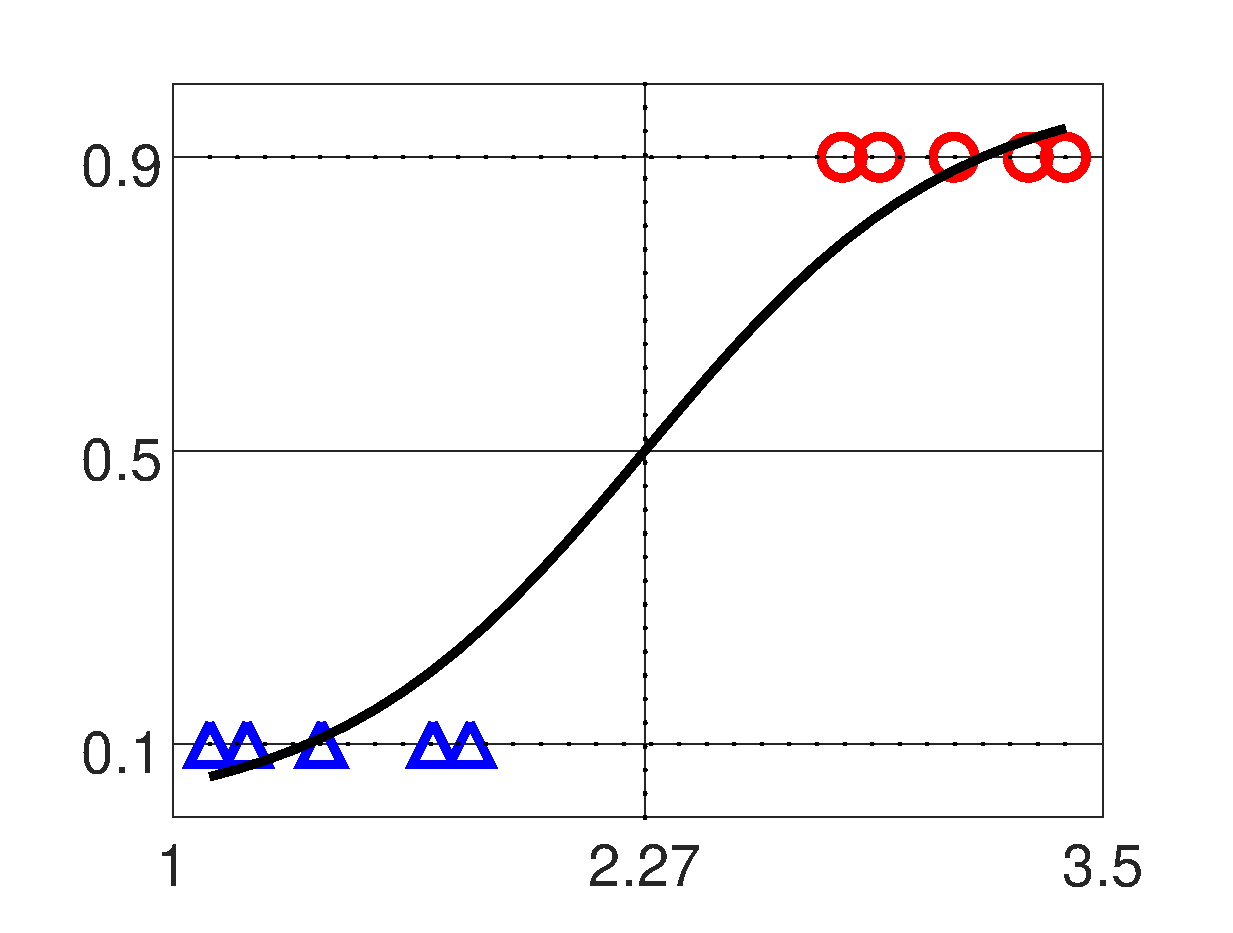
\includegraphics[width=\textwidth]{chapters/classificacao/mfiles/reglogr1r1/ex1s1-reglogr1r1.eps}
        \caption{Gráfico da classificação usando $y_l \in \{0.1,~ 0.9\}$.}
        \label{fig:theo:reglogr1r1:xn:s1}
    \end{subfigure}
    \hfill
    \begin{subfigure}[b]{0.45\textwidth}
        \centering
        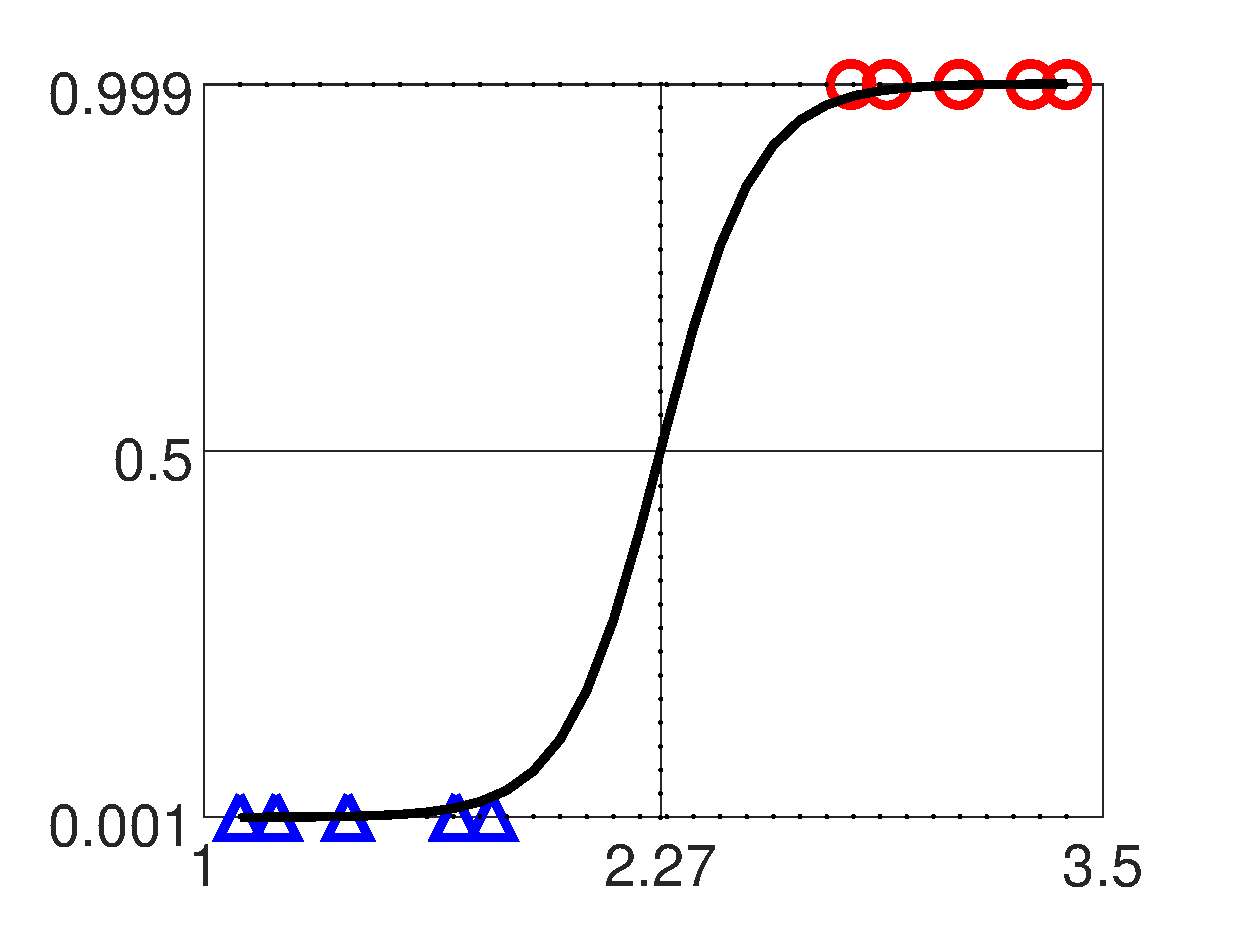
\includegraphics[width=\textwidth]{chapters/classificacao/mfiles/reglogr1r1/ex1s2-reglogr1r1.eps}
        \caption{Gráfico da classificação usando $y_l \in \{0.001,~ 0.999\}$.}
        \label{fig:theo:reglogr1r1:xn:s2}
    \end{subfigure}
    \caption{Classificação usando a função $f_{\VECTOR{c}}(x)$.}
    \label{fig:theo:reglogr1r1:xn}
\end{figure}


\begin{SolutionT}[Relativa ao Exemplo \ref{ex:theo:reglogr1r1}:]\label{sol:theo:reglogr1r1:s2}
Para obter o vetor de parâmetros $\VECTOR{c}=\VECTOR{\hat{c}}$ da função $f_{\VECTOR{c}}(x)$, 
que gere o menor erro $e(\VECTOR{c}) =  \sum_{l=1}^{L} ||c_1 +c_2 x_l-logit(y_l)||^2$
com os $L=10$ dados $x_l$ da Tabela \ref{table:theo:reglogr1r1:xn},
usamos a Eq. (\ref{eq:reglogr1r1:2}) onde escolhemos $w_l=1$ e valores $y_l \in \{0.001,~ 0.999\}$,
$0.001$ para $\bigtriangleup$ e $0.999$ para $\bigcirc$,
obtendo um vetor $\VECTOR{\hat{c}}=[-17.3022\quad 7.6221]^{\transpose}$. 
Assim, podemos representar a função $\left.f_{\VECTOR{c}}(x)\right|_{\VECTOR{c}=\VECTOR{\hat{c}}}$ que classifica os dados $x_l$, 
como é mostrado na Figura \ref{fig:theo:reglogr1r1:xn:s2}  e na Eq. (\ref{eq:theo:reglogr1r1:xn:s2}),
\begin{equation}\label{eq:theo:reglogr1r1:xn:s2}
f_{\VECTOR{\hat{c}}}(x)= \frac{1}{1+e^{ 17.3022-7.6221 x}}.
\end{equation}
É interessante ressaltar que para um valor $A=0.001$ a pendente é abrupta para cada grupo e a classificação é bem definida,
com limiar de classificação em $2.27$.
\end{SolutionT}

\index{Gauss, Karl Friedrich }
\begin{elaboracion}[title=Karl Friedrich Gauss (1777-1855), width= 0.99\linewidth]
\label{elab:Gauss}
\noindent
Notável matemático, astrônomo e físico alemão;
o jovem Gauss achou a formula $\sum_{n=1}^{N}n=\frac{N(N+1)}{2}$.
Na sua etapa adulta estudou no ``Caroline College'' em Brunswick (1792-1795)
e posteriormente na ``University of G\"ottingen'' (1795-1798).
Entre suas contribuições à matemática podemos mencionar 
a minimização do erro nos dados observados
 mediante o método de mínimos quadrados \cite[pp. 225]{agarwal2014creators}.
\end{elaboracion}
